%
%  A presentation of ZMailer for  FUUG at SEA 2000 conference
%
%     FUUG = Finnish Unix User Group
%     SEA  = The baltic sea; cruising from Helsinki to Stockholm, and back
%
%  Matti Aarnio, 12-Sep-2000
%

\documentclass[a4paper,landscape]{slides}

\setlength{\topmargin}{-40pt}
\setlength{\headsep}{2EM}
\setlength{\footskip}{3\footskip}

\usepackage[dvips]{color}
\usepackage[dvips]{epsfig}
\usepackage{wrapfig}

\newcommand{\SLIDEFOOT}{\centerline{\rm Matti Aarnio $<matti.aarnio@sonera.fi>$}\hfil\theslide}
\newcommand{\SLIDEHEAD}{\centerline{\tiny\rm FUUG @ SEA-2000:   ZMailer}}

\newcommand{\ZM}{ZMailer}

\begin{document}
\pagestyle{plain}

%%%%%%%%%%%%%%%%%%%%%%%%%%%%%%%%%%%%%%%%%%%%%%%%%%%%%%%%%%%%%%%%%

\begin{slide}

\begin{center}
 ZMailer --- A Different Kind of MTA
\end{center}

\vfill

\begin{center}
 
\epsfig{file=zmailer-logo.ps}
\end{center}

\vfill

\end{slide}

%%%%%%%%%%%%%%%%%%%%%%%%%%%%%%%%%%%%%%%%%%%%%%%%%%%%%%%%%%%%%%%%%

\begin{overlay}

\begin{center}
 ZMailer --- A Different Kind of MTA
\end{center}

\vfill

  A presentation of ZMailer for  FUUG at SEA 2000 conference

     FUUG = Finnish Unix User Group

     SEA  = The baltic sea; cruising from Helsinki to Stockholm, and back

 Matti Aarnio, 12-Sep-2000


\end{overlay}

%%%%%%%%%%%%%%%%%%%%%%%%%%%%%%%%%%%%%%%%%%%%%%%%%%%%%%%%%%%%%%%%%


\begin{slide}
\centerline{\large A bit of History}

\vfill
\ZM{} was created at {\it University of Toronto} around 1986 by
Mr. {\it Rayan Zachariassen} (hence the ``Z'' in the name.)

Rayan went to private sector around 1992, and $ZMailer$ development
was essentially abandoned by him.

Since then, yours truly has been hacking at it developing all kinds
of extensions for modern Internet email.

\vfill

\end{slide}

%%%%%%%%%%%%%%%%%%%%%%%%%%%%%%%%%%%%%%%%%%%%%%%%%%%%%%%%%%%%%%%%%


\begin{slide}

\centerline{\large \ZM{} structure}

\begin{wrapfigure}{l}{3in}
\mbox{
   \epsfig{file=zmprocs.ps,width=2.7in}
\\
}
\end{wrapfigure}

\ZM{} consists of several main subsystems running in coordinated,
although separate existence.  This means also that any of the subsystems
can be shut down for a while without harming other subsystem functionality.

The task-transfer in between the subsystems is done via
the filesystem -- {``\it spool''}.

\vfill
\centerline{\it There are no suid-anything programs in this system!}

\vfill

\end{slide}

%%%%%%%%%%%%%%%%%%%%%%%%%%%%%%%%%%%%%%%%%%%%%%%%%%%%%%%%%%%%%%%%%


\begin{slide}

\centerline{\large \ZM{} subsystems: {\it ``POSTOFFICE/''}}

The \verb!$POSTOFFICE/! is \ZM{}'s way of referring to filesystem
where a few basic things are guaranteed to happen:
\begin{enumerate}
\item moving files around with {\it rename(2)} and/or {\it link(2), unlink(2)}
      works just fine in between different directories
\item i-node numbers are preserved over {\it rename(2)}, and {\it link(2)}
	system calls
\end{enumerate}

There are filesystems where these two things don't happen, e.g. possibly
{\it link(2)} can't be done in between directories.  Such ones are not
suitable for \ZM's \verb!$POSTOFFICE/! partition use.
\vfill

\end{slide}

%%%%%%%%%%%%%%%%%%%%%%%%%%%%%%%%%%%%%%%%%%%%%%%%%%%%%%%%%%%%%%%%%


\begin{slide}

\centerline{\large \ZM{} subsystems: {\it ``sendmail''}}

For normal local system use there needs to be a well-known
submission interface for email.  A de-facto one is {\it sendmail.}

\ZM's {\it sendmail} implements most of message submission options
of the real {\it sendmail(8).}

Many of {\it sendmail(8)} options are meaningless in \ZM{}, and thus
they are ignored, or in case of several administrative functions,
start subsystems in interactive test mode and/or just plain complain
loudly.

For message submission, \ZM's {\it sendmail} is extremely
{\it lightweight} one.  Just writing the message envelope and
message to the file, and moving it to {\it router} subsystem's care.



\vfill

\end{slide}

%%%%%%%%%%%%%%%%%%%%%%%%%%%%%%%%%%%%%%%%%%%%%%%%%%%%%%%%%%%%%%%%%


\begin{slide}

\centerline{\large \ZM{} subsystems: {\it ``smtpserver''}}

\begin{wrapfigure}{l}{5in}
\tiny
\begin{tabular}{ll}
ESMTP RFC's \\
1425/1651/2045 & EHLO framework \\
1426/1652 & 8BITMIME \\
1427/1653/1870 & SIZE \\
1830 & CHUNKING \\
1854/2197 & PIPELINING \\
1891 & DSN \\
1985 & ETRN \\
2034 & ENHANCEDSTATUSCODES \\
2487 & STARTTLS \\
2554+MS & AUTH LOGIN \\
2554+Netscape & AUTH=LOGIN
\end{tabular}
\end{wrapfigure}
\ZM's {\it smtpserver} subsystem implements a rich set of enhanced SMTP
features defined over the last 10 or so years.

At the same time it aims to be lightweight, fast protocol receiver with
ability to quickly verify incoming protocol stream syntax conformance,
but it can also be configured to behave sloppily in this regard.

\vfill

\end{slide}

%%%%%%%%%%%%%%%%%%%%%%%%%%%%%%%%%%%%%%%%%%%%%%%%%%%%%%%%%%%%%%%%%


\begin{slide}

\centerline{\large \ZM{} subsystems: {\it ``smtpserver''} (2)}

\ZM's {\it smtpserver} can be configured to process fairly simple
access-control tests at the incoming addresses in order to avoid
email relaying abuse thru the server.

\ZM's {\it smtpserver} is one of the first open source servers
capable of speaking TLS encryption on the connection.
This enables a bit less nervousness when sending ESMTP user AUTHentication
for message submission by using de-factor ``LOGIN'' method.

Also several non-lightweight testing facilities can be hooked into
message reception, e.g. synchronous router subsystem usage for
SMTP envelope address analysis, and arrived message content scanning
at the reception time with an external program.

%\vfill

\end{slide}

%%%%%%%%%%%%%%%%%%%%%%%%%%%%%%%%%%%%%%%%%%%%%%%%%%%%%%%%%%%%%%%%%


\begin{slide}

\centerline{\large \ZM{} subsystems: {\it ``router''}}

\vfill

\end{slide}

%%%%%%%%%%%%%%%%%%%%%%%%%%%%%%%%%%%%%%%%%%%%%%%%%%%%%%%%%%%%%%%%%


\begin{slide}

\centerline{\large \ZM{} subsystems: {\it ``scheduler''}}

\vfill

\end{slide}

%%%%%%%%%%%%%%%%%%%%%%%%%%%%%%%%%%%%%%%%%%%%%%%%%%%%%%%%%%%%%%%%%


\end{document}
